\documentclass[a4paper,12pt]{report}

\usepackage{amsfonts}
\usepackage{mathptmx}
\usepackage{amssymb}
\usepackage{microtype}
\usepackage{graphicx}
\usepackage{wrapfig}
\usepackage{enumitem}
\usepackage{fancyhdr}
\usepackage{index}
\usepackage{keyval}
\usepackage[italian]{babel}
\usepackage[font=small,labelfont=bf]{caption}
\usepackage{tikz, pgfplots}
\usepackage{blindtext}
\usepackage{caption}
\usepackage{subcaption}
\usepackage{amsmath}
\usepackage{cancel}
\usepackage{epigraph}

\begin{document}

\title{\textbf{Da Cartesio a Philip Glass}}
\author{di Salvatore Palumbo}
\date{16 Giugno 2021}
\maketitle

\thispagestyle{empty}
\vspace*{\fill}
\parbox{110mm}{\setlength{\epigraphwidth}{0.8\textwidth}
               \epigraph{\textbf{Truman:} Chi sei tu? \\
                         \textbf{Christof:} Sono il creatore... di uno show televisivo che dà speranza, gioia ed esalta milioni di persone.\\
                         \textbf{Truman:} E io chi sono?\\
                         \textbf{Christof:} Tu sei la star!\\
                         \textbf{Truman:} Non c'era niente di vero?\\
                         \textbf{Christof:} Tu eri vero! Per questo era così bello guardarti. Ascoltami Truman, là fuori non troverai più verità di quanta non ne esista nel mondo che ho creato per te... le stesse ipocrisie, gli stessi inganni; ma nel mio mondo tu non hai niente da temere... Io ti conosco meglio di te stesso!\\
                         \textbf{Truman:} Non ho una telecamera nella testa!\\
                         \textbf{Christof:} Tu hai paura... per questo non puoi andare via. Stai tranquillo... ti capisco. Ho seguito ogni istante della tua vita. Ti ho seguito quando sei nato. Ti ho seguito quando hai mosso i tuoi primi passi. Ti ho seguito nel tuo primo giorno di scuola. Il momento in cui hai perso il tuo primo dentino... come fai ad andartene? Il tuo posto è qui, con me! Dai... dì qualcosa... accidenti Truman, vuoi parlare?, siamo in televisione! Sei in diretta mondiale!\\
                         \textbf{Truman:} Buongiorno... e casomai non vi rivedessi, buon pomeriggio, buonasera e buonanotte!
                         }{\textit{The Truman Show, Peter Weir, 1998}}}
\vfill

\tableofcontents


\pagenumbering{Roman}
\setcounter{page}{3}

\chapter{La nascita dell'analisi}


\section{Gli assi cartesiani}
\paragraph{Storia} 
La prima rappresentazione della realtà mediante coordinate geometriche avvenne nel XIV secolo d.C. da parte del matematico francese Nicola d’Oresme (1323-1382). Come riportato nella sua opera più importante il “Tractatus de configuratione qualitatum et motuum“, Orseme ebbe l’intuizione di utilizzare le cosiddette \textit{coordinate rettangolari} della terminologia moderna, una lunghezza proporzionale alla longitudo, l’ascissa di un dato punto e una perpendicolare a quel punto, proporzionale alla latitudo, l’ordinata. Oresme mostrò che la proprietà geometrica di una tale figura potrebbe essere considerata come corrispondente ad una proprietà della forma stessa. I parametri longitudo e latitudo possono variare o rimanere costanti\cite{Oresme}.

\begin{wrapfigure}{r}{0.4\textwidth}
  \centering
    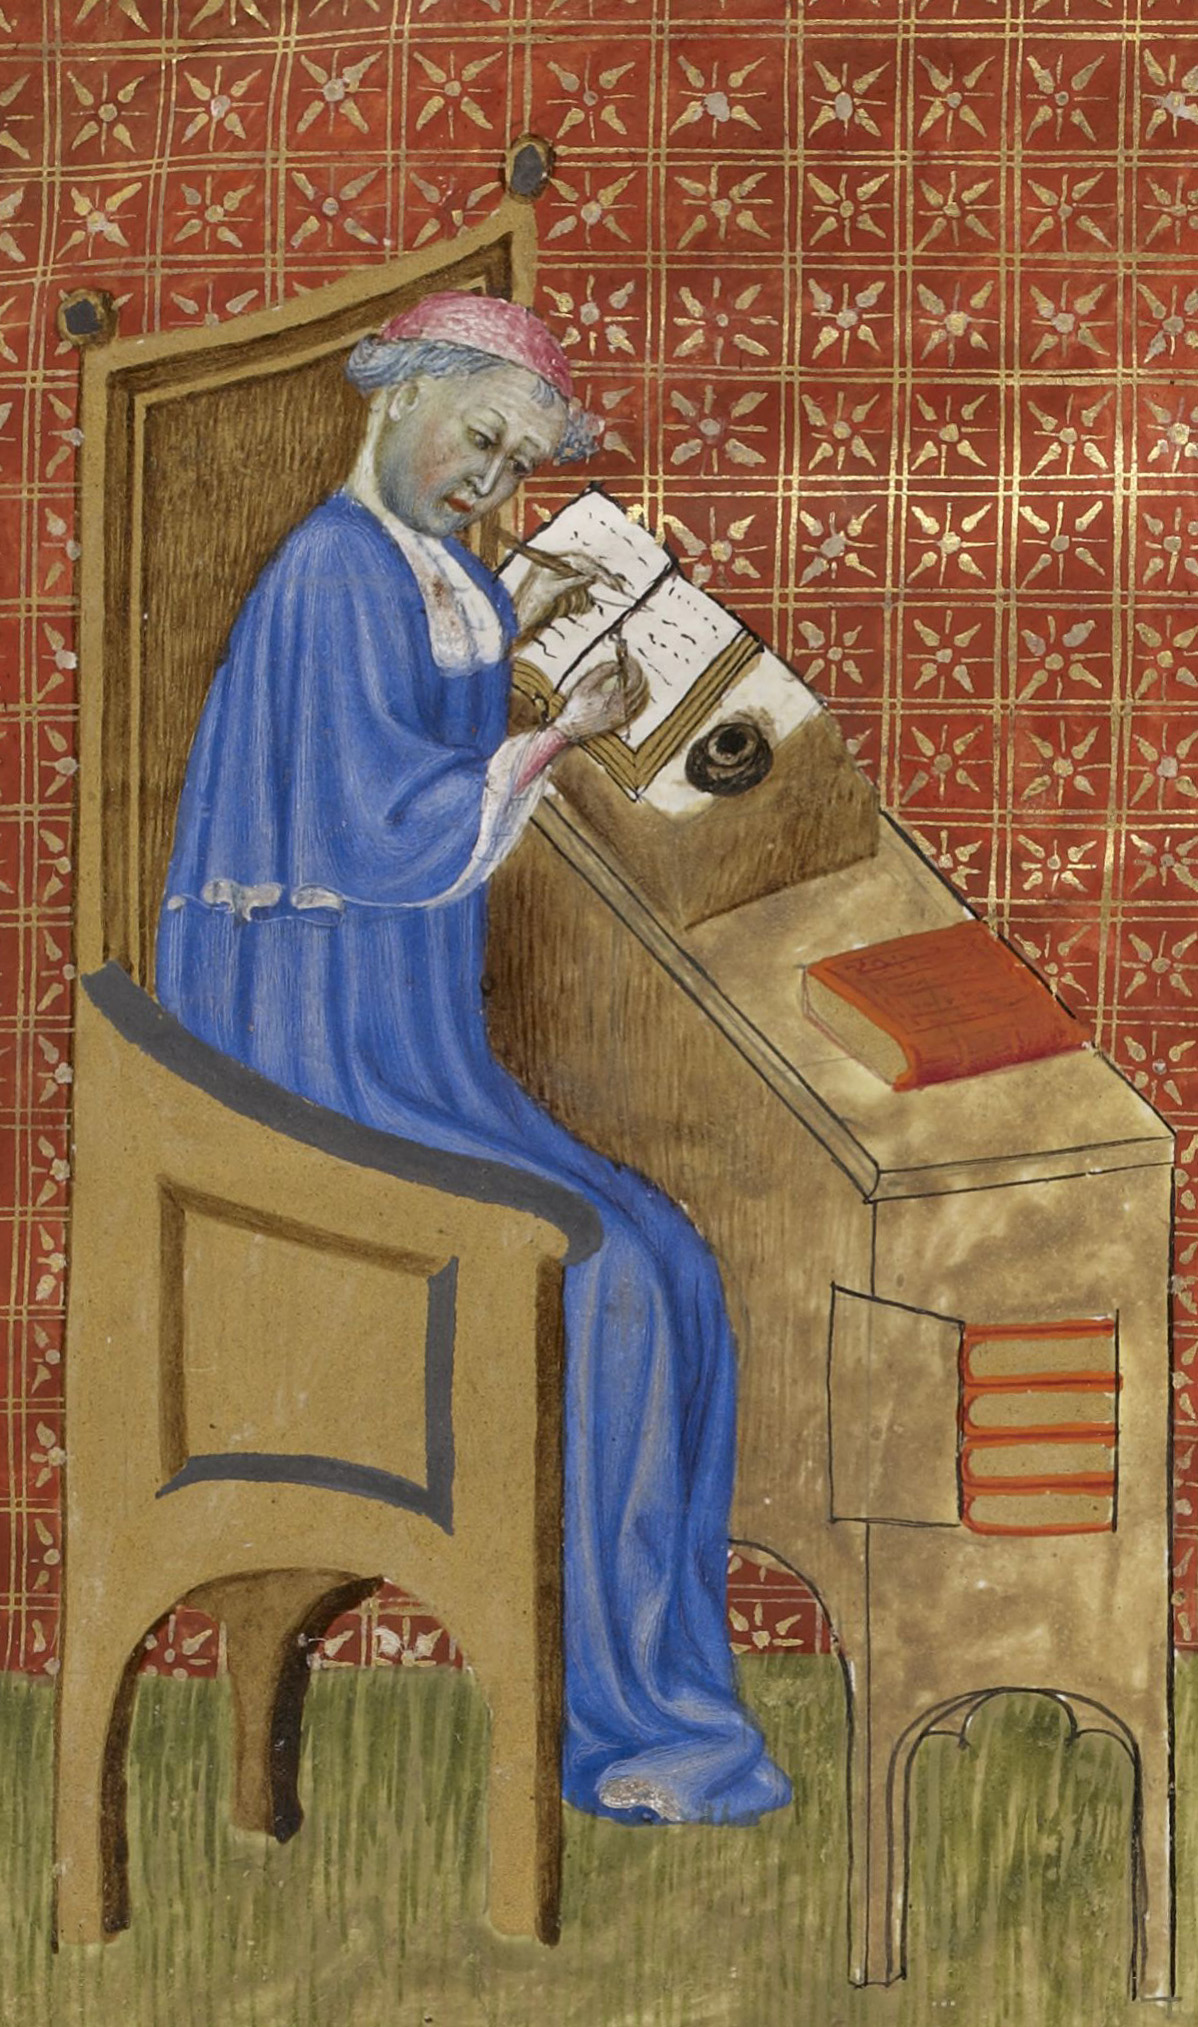
\includegraphics[width=0.22\textwidth]{Oresme-Nicole.jpg}
  \caption{Nicole d'Oresme}

\end{wrapfigure}
Inoltre dimostrò che questa definizione è sintetizzabile attraverso un’ espressione algebrica in cui compaiono “longitudini” e “latitudini”di ogni terna di punti, ottenendo così l’equazione della retta e anticipando di molto Cartesio nell’invenzione della geometria analitica. \\
Dalla morte di D’Oresme (1382) alla nascita di Cartesio (1596) passano 214 anni. Le scoperte di d’Oresme sedimentano, vengono discusse, elaborate, ma nessuno riesce a renderle un vero sistema prima di Cartesio. \\
René Descartes (1596-1650), noto nella sua traduzione in latino come Renatus Cartesius, da cui anche il nome “assi cartesiani” costituisce assieme a Galileo Galilei (1564-1642) e Pierre de Fermat
(1601-1665) uno dei 

\begin{wrapfigure}{l}{0.4\textwidth}
  \centering
    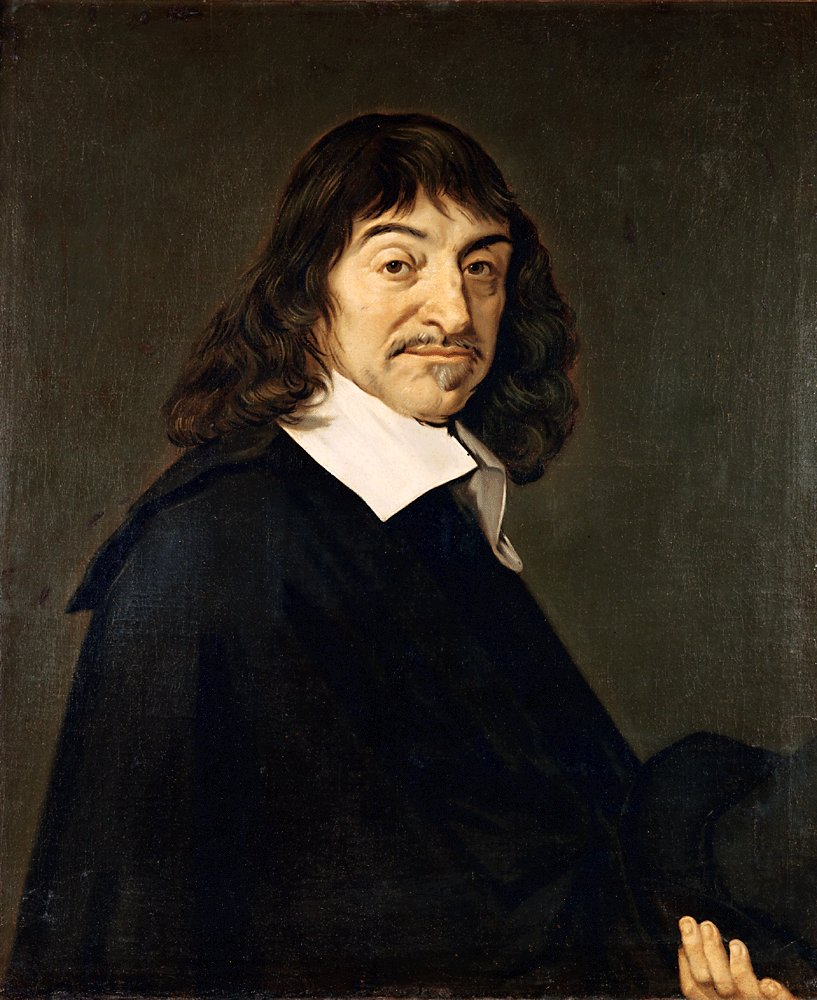
\includegraphics[width=0.21\textwidth]{Frans_Hals_-_Portret_van_René_Descartes.jpg}
  \caption{René Descartes}
\end{wrapfigure}
capisaldi della matematica occidentale. In particolare Cartesio a differenza dei suoi predecessori pone per la prima volta al centro della conoscenza le \textit{matematiche} “per la certezza e l’evidenza dei loro ragionamenti”. Essa non costituisce un sapere \textit{unitario} e \textit{coerente}, ma uno strumento adoperato \textit{per le arti meccaniche}\cite{Metodo}, che condurrà alla nascita della geometria analitica e alla completa matematizzazione delle realtà dimensionali.


\paragraph{Un nuovo modo di vedere il mondo}
Cartesio consentì alla scienza di compiere un passo ulteriore a quello fatto da Galileo con l’introduzione del metodo sperimentale. Difatti Cartesio aveva fornito alle scienze lo strumento essenziale per la rappresentazione del mondo su di un modello, la \textit{mathesis universalis}. Tuttavia Cartesio distingueva due tipi di scienze, quelle come la fisica legate alla \textit{res extensa}, ovvero la materia tangibile, misurabile, quantitativamente discreta, e quelle legate alla \textit{res cogitans} come la Teologia e la metafisica. Questa concezione perdurò per almeno due secoli fino a quando con l’illuminismo e soprattutto con Immanuel Kant si abbandonò il concetto di metafisica e si sarebbe aperto di lì a poco la strada al meccanicismo e al positivismo moderno.
Il metodo proposto da Cartesio in realtà era in grado di risolvere tutte le scienze i cui principi derivassero dalla filosofia. Essa va infatti immaginata \textit{come un albero, di cui le radici sono la  metafisica, il tronco è la fisica, e i rami che sorgono da questo tronco sono tutte le altre scienze, che si riducono a tre principali, cioè la medicina, la meccanica e la morale}.
Tuttavia la solidità di questo sistema si fonda sulla solidità della filosofia stessa, ed è quindi necessario anzitutto stabilire alcuni principi nella filosofia. Cartesio, allora affronta questo problema  adottando il procedimento del \textit{dubbio metodico}\cite{metameditazioni}: si tratta di mettere in dubbio tutte le nostre \textit{idee evidenti}, sensibili e intelligibili, alla ricerca di una che conservi i caratteri dell’assoluta certezza. Non è scetticismo, in quanto il fine non è la distruzione del concetto di verità ma un mezzo per condurci ad essa.
In quest’ottica per Cartesio non dovrebbe esistere “l’errore” in quanto il criterio della verità, della chiarezza e distinzione, dell'evidenza, garantito dal \textit{cogito ergo sum} e dalla esistenza dimostrata razionalmente di un Dio perfetto, buono, quindi veridico dovrebbe rendere, secondo Cartesio, impossibile l'errore. Difatti l’errore che talvolta commettiamo nel giudicare \textit{evidente} un’ idea che invece è \textit{confusa} è dovuto a qualcosa di esterno al pensiero, costituito dalla volontà. Non che l’uomo sbagli volontariamente, ma che ci sia una forza esterna, la volontà appunto, che ci induce all’errore. Un po’ come succede con le \textit{passioni}, come l’amore, provocato da un \textit{movimento degli spiriti}, che incita l’anima a desiderare il congiungimento con gli oggetti che le sembrano convenienti, oltrepassando le barriere imposte dal pensiero\cite{passioni}.


\paragraph{Definizione di assi cartesiani}
\begin{wrapfigure}{l}{0.23\textwidth}
  \centering
    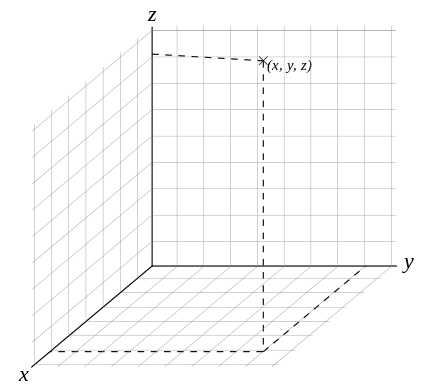
\includegraphics[width=0.2\textwidth]{Cartesian_with_grid.svg.png}
  \caption{Sistema cartesiano a tre dimensioni}
\end{wrapfigure}
Un piano cartesiano non è altro che un sistema di coordinate cartesiane ortogonali in due dimensione. Una catena di piani cartesiani lungo un terzo asse forma un sistema cartesiano a tre dimensioni. Formalmente si è soliti indicare con x,y,z i tre assi ortogonali e per ogni piano cartesiano si distinguono 4 quadranti numerati in senso antiorario partendo da quello in alto a destra.
L’intersezione degli assi viene generalmente detta O e ha coordinate O(0;0), qualsiasi punto (a;b) che si trova nel primo o nel terzo quadrante ha coordinate rispettivamente sempre positive o sempre negative, mentre se si trova nel secondo quadrante ha coordinata a negativa e b positiva e se si trova nel quarto ha coordinate a positiva e b negativa.
Un sistema cartesiano permette la rappresentazione geometrica di qualsiasi equazione algebrica, permettendo quindi la fusione tra le due discipline. 
Per esempio l’espressione algebrica $x^{2} + y^{2} = 4$ racchiude in se tutte le coordinate (x;y) che disegnate su di un piano cartesiano costituiscono l’equazione di una circonferenza di raggio 2 e centro in O. Sono i fondamenti della geometria analitica, che seppur tenendo fede ai 5 postulati di Euclide, inquadra lo spazio in un altro modo al fine di legare indossulubilmente astratto(algebra) e concreto(figure geometriche).\\
\begin{figure}[h]
\begin{center}
\begin{tikzpicture}
	  \begin{axis}[ 
	    width=0.56\textwidth,
	    height=0.56\textwidth,
	    samples=100,      
	    axis x line=center,
	    axis y line=center,
	    xtick={-5,-4,...,5},
	    ytick={-5,-4,...,5},
	    xlabel=$x$,
	    ylabel={$y$},
	    xlabel style={below right},
	    ylabel style={above left},
	    xmin=-5.5,
	    xmax=5.5,
	    ymin=-5.5,
	    ymax=5.5,
	    smooth,
	    yticklabels={,,},
	    xticklabels={,,},
	  ] 
	    \addplot [mark=none, domain=-2:2]{sqrt(-x^2 +4)};
	    \addplot [mark=none, domain=-2:2]{-sqrt(-x^2 +4)};
	  \end{axis}
	\end{tikzpicture}
	\caption{Circonferenza}
\end{center}
\end{figure}



\section{Funzione}
\paragraph{Definizione}
Una funzione è un caso particolare di corrispondenza tra gli elementi di un insieme A e gli elementi di un insieme B. La condizione necessaria affinché questa corrispondenza sia una funzione è che ogni elemento dell’insieme A non leghi più di un elemento nell’insieme B. Tuttavia, è possibile l’inverso, ovvero che più elementi dell’insieme A abbiano la stessa immagine in B.
Formalmente tutto ciò si traduce come: \\
\begin{center}
$\forall a\; \in\;  A\; \exists !\; b\; \in\; B\;\;\;\;tale\; che\;\;\;\; f   : a \to b$ 
\end{center} 
\begin{figure}[h]
\begin{subfigure}{0.5\textwidth}
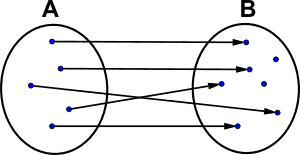
\includegraphics[width=0.42\linewidth,]{esempio-di-funzione-1.png}
\caption{Funzione inniettiva}
\end{subfigure}
\begin{subfigure}{0.5\textwidth}
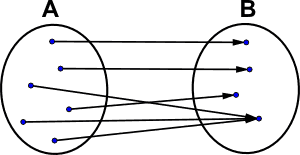
\includegraphics[width=0.42\linewidth]{esempio-di-funzione-2.png}
\caption{Funzione non inniettiva}
\end{subfigure}
\begin{center}
\begin{subfigure}{0.5\textwidth}
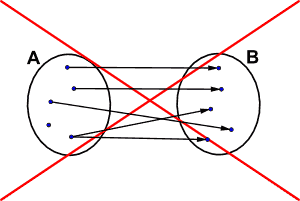
\includegraphics[width=0.54\linewidth]{esempio-di-non-funzione.png}
\caption{Non funzione}
\end{subfigure}
\end{center}
\caption{Esempi di funzioni e non funzioni}
\end{figure}
In generale si è soliti assegnare una nomenclatura specifica agli elementi coinvolti in una funzione.
Se un elemento $b \in B$ ha una corrispondenza che parte da un elemento $a \in A$ mediante la funzione $f$ \\
\begin{center}
$f   : a \to b$ 
\end{center}
allora scriviamo: \\
\begin{center}
$f(a)\; =\; b$
\end{center}
e chiamiamo:
\begin{itemize}
\item {$b$ l’immagine di $a$ mediante la funzione $f$}
\item {$a$ la controimmagine di $b$ mediante $f$}
\end{itemize}
L’insieme A prende il nome di dominio, che corrisponde all’insieme di definizione della funzione $f$, mentre l’insieme B prende il nome di codominio, e il sottogruppo di B corrispondente agli elementi che hanno una corrispondenza con A prende il nome di immagine.\\
In genere le funzioni di cui ci interessiamo sono le funzioni reali a variabile reale , ovvero le funzioni in cui il dominio è costituito da $R$ o un suo sottoinsieme, e il codominio è costituito da tutto $R$ (l’immagine può essere anche un suo sottoinsieme).

\section{Derivate}
\paragraph{Derivata in un punto}
La derivata in un punto è un operatore matematico che nasce per sopperire al problema del calcolo del coefficiente angolare della retta tangente in un punto di una funzione $f(x)$. 
Se consideriamo una secante che taglia una curva  in due punti con $\Delta x\;=\;h$, il limite per $h$ che tende a $0$ del rapporto incrementale $\frac{\Delta y}{\Delta x}$ ci riconduce geometricamente alla tangente in quel punto della funzione. Algebricamente tutto ciò si traduce come: \\
\begin{center}
$\lim_{h\to 0}\frac{\Delta y}{\Delta x}\; =\; \lim_{h\to 0}\frac{f(x_{0}+h)-f(x_{0})}{h}\;=\; \tan(\beta)\;=\;f’(x_{0})$
\end{center}
\medskip 
Una funzione si dice derivabile in un punto $x_{0}$ sse esiste il limite sopra citato ed è finito.
\medskip
\begin{figure}[h]
\centering
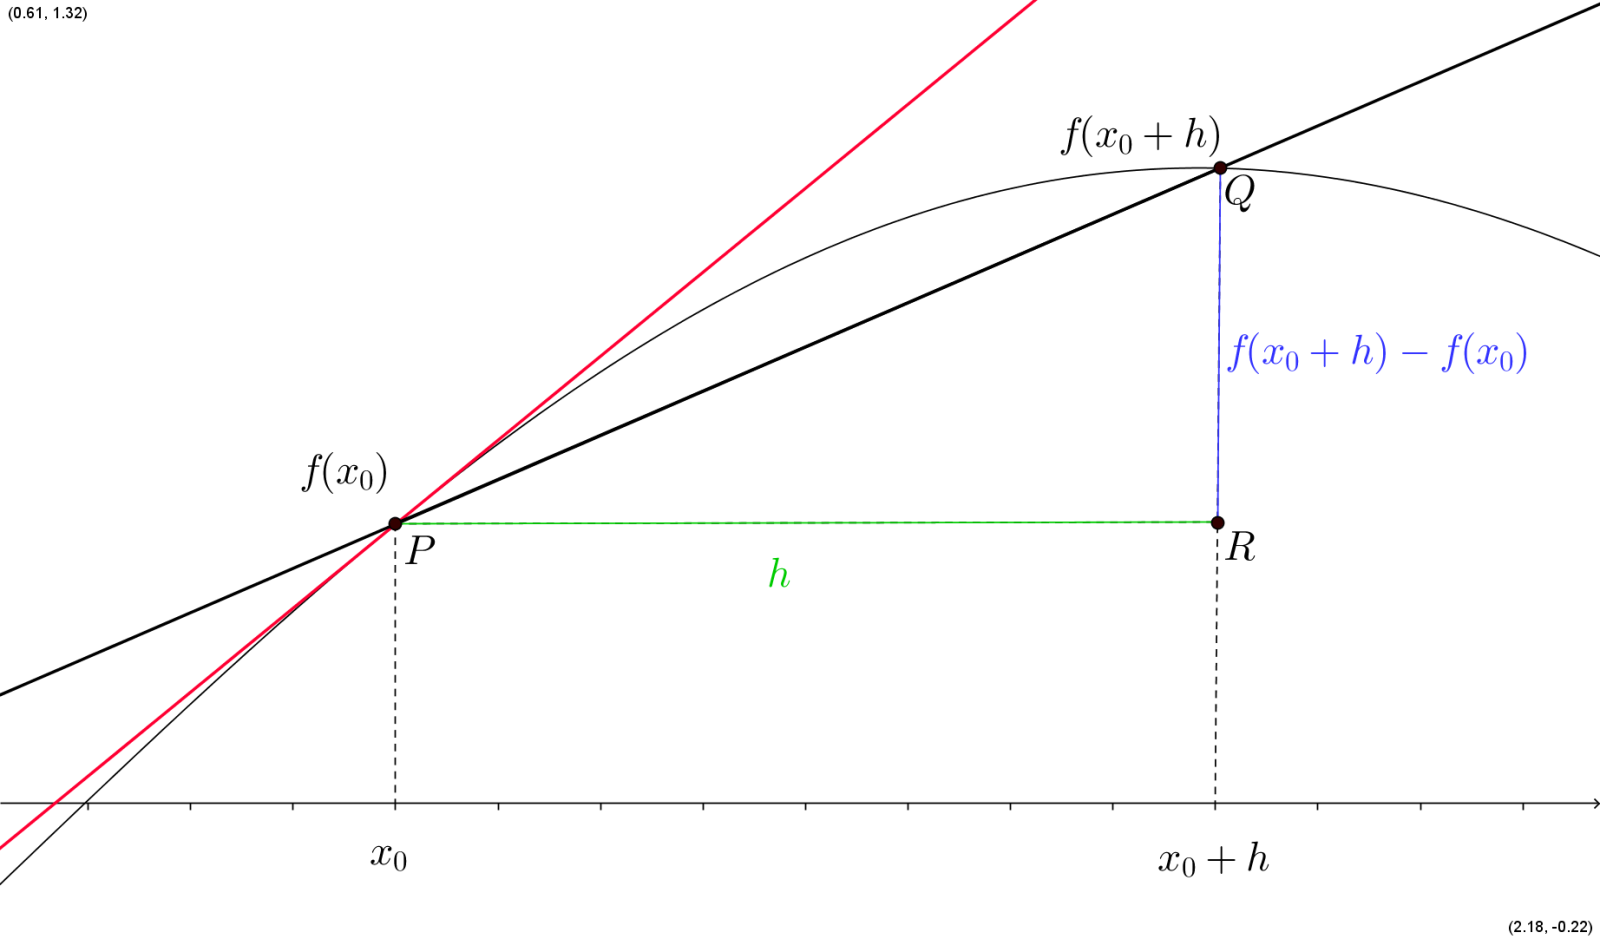
\includegraphics[scale=0.22]{disegno_PQR.png}
\caption{Interpretazione geometrica}
\end{figure}

\paragraph{Punti di non derivabilità}
Ovviamente una funzione non può essere derivabile sempre in tutto i suoi punti. Tralasciando le discontinuità che in quanto tali non possono essere ivi derivabili, esistono dei punti che appartengono al dominio $D$ della funzione ma che presentano delle derivate indefinite prendendo il nome per l’appunto di punti di non derivabilità. 
Essi si classificano in : \\
\begin{enumerate}
\item {Flesso discendente a tangente verticale}\\
In genere i flessi sono dei punti in cui nella funzione c’è un’ inversione di concavità, e ne esistono di tre tipi: a tangente verticale, obliqua e orizzontale. Tra questo solo i primi si definiscono punti di non derivabilità e in particolare quelli discendenti sono i flessi nei quali la concavità passa da rivolta verso l’alto a rivolta verso il basso.
In questo punto la derivata da destra e quella da sinistra sono uguali a: \\
\begin{center}
$\lim_{x\to x_{0^-}}\frac{f(x) – f(x_{0})}{x-x_{0}} \;=\; +\infty$ \qquad
$\lim_{x\to x_{0^+}}\frac{f(x) – f(x_{0})}{x-x_{0}} \;=\; +\infty$
\end{center}
\textbf{Esempio:} \\

\begin{center}
\begin{equation}
	 f(x) = 
      \begin{cases}
        -\sqrt{-2x} & \text{se}\;\; x < 0\\
        \sqrt{2x} & \text{se}\;\; x \geq 0
      \end{cases}\,.
\end{equation}
\end{center}

\begin{figure}[!h]
\begin{center}
\begin{tikzpicture}
	  \begin{axis}[ 
	    width=0.48\textwidth,
	    height=0.48\textwidth,
	    samples=200,      
	    axis x line=center,
	    axis y line=center,
	    xtick={-8,-7,...,8},
	    ytick={-8,-7,...,8},
	    xlabel=$x$,
	    ylabel=$f(x)$,
	    xlabel style={below right},
	    ylabel style={above left},
	    xmin=-8.5,
	    xmax=8.5,
	    ymin=-8.5,
	    ymax=8.5,
	    smooth,
	    yticklabels={,,},
	    xticklabels={,,},
	  ] 
	    \addplot [mark=none, domain=0:7]{sqrt(2*x)};
	    \addplot [mark=none, domain=-7:0]{-sqrt(-2*x)};
	  \end{axis}
	\end{tikzpicture}
	\caption{Flesso discendente a tangente verticale in $x_{0} = 0$}
\end{center}
\end{figure}
\newpage

\item {Flesso ascendente a tangente verticale}\\
Così come per il flesso discendente anche quello ascendente rappresenta un punto di non derivabilità in cui la concavità passa da rivolta verso il basso a rivolta verso l’alto.
In questo punto la derivata da destra e quella da sinistra sono uguali a: \\
\begin{center}
$\lim_{x\to x_{0^-}}\frac{f(x) – f(x_{0})}{x-x_{0}} \;=\; -\infty$ \qquad
$\lim_{x\to x_{0^+}}\frac{f(x) – f(x_{0})}{x-x_{0}} \;=\; -\infty$
\end{center}
\textbf{Esempio:} \\

\begin{center}
\begin{equation}
	 f(x) = 
      \begin{cases}
        \sqrt{-2x} & \text{se}\;\; x < 0\\
        -\sqrt{2x} & \text{se}\;\; x \geq 0
      \end{cases}\,.
\end{equation}
\end{center}

\begin{figure}[!h]
\begin{center}
\begin{tikzpicture}
	  \begin{axis}[ 
	    width=0.48\textwidth,
	    height=0.48\textwidth,
	    samples=200,      
	    axis x line=center,
	    axis y line=center,
	    xtick={-8,-7,...,8},
	    ytick={-8,-7,...,8},
	    xlabel=$x$,
	    ylabel=$f(x)$,
	    xlabel style={below right},
	    ylabel style={above left},
	    xmin=-8.5,
	    xmax=8.5,
	    ymin=-8.5,
	    ymax=8.5,
	    smooth,
	    yticklabels={,,},
	    xticklabels={,,},
	  ] 
	    \addplot [mark=none, domain=0:7]{-sqrt(2*x)};
	    \addplot [mark=none, domain=-7:0]{sqrt(-2*x)};
	  \end{axis}
	\end{tikzpicture}
	\caption{Flesso ascendente a tangente verticale in $x_{0} = 0$}
\end{center}
\end{figure}

\item {Cuspide a vertice rivolto verso il basso}\\
Le cuspidi sono punti di non derivabilità simmetrici che non presentano inversione di concavità. La loro derivata da destra e da sinistra sono uguali a: \\
\begin{center}
$\lim_{x\to x_{0^-}}\frac{f(x) – f(x_{0})}{x-x_{0}} \;=\; -\infty$ \qquad
$\lim_{x\to x_{0^+}}\frac{f(x) – f(x_{0})}{x-x_{0}} \;=\; +\infty$
\end{center}

\textbf{Esempio:} \\

\begin{center}
\begin{equation}
	 f(x) = 
      \begin{cases}
        \sqrt{-x^2 -4x} & \text{se}\;\;-2 \leq x < 0\\
        \sqrt{-x^2 +4x} & \text{se}\; \quad 0 \leq x \leq 2
      \end{cases}\,.
\end{equation}
\end{center}

\begin{figure}[!h]
\begin{center}
\begin{tikzpicture}
	  \begin{axis}[ 
	    width=0.48\textwidth,
	    height=0.48\textwidth,
	    samples=200,      
	    axis x line=center,
	    axis y line=center,
	    xtick={-8,-7,...,8},
	    ytick={-8,-7,...,8},
	    xlabel=$x$,
	    ylabel=$f(x)$,
	    xlabel style={below right},
	    ylabel style={above left},
	    xmin=-8.5,
	    xmax=8.5,
	    ymin=-8.5,
	    ymax=8.5,
	    smooth,
	    yticklabels={,,},
	    xticklabels={,,},
	  ] 
	    \addplot [mark=none, domain=-2:0]{sqrt(-x^2 -4*x)};
	    \addplot [mark=none, domain=0:2]{sqrt(-x^2 +4*x)};
	  \end{axis}
	\end{tikzpicture}
	\caption{Cuspide a vertice rivolto verso il basso in $x_{0} = 0$}
\end{center}
\end{figure}

\item {Cuspide a vertice rivolto verso l’alto}\\
La loro derivata da destra e da sinistra  sono uguali a: \\
\begin{center}
$\lim_{x\to x_{0^-}}\frac{f(x) – f(x_{0})}{x-x_{0}} \;=\; +\infty$ \qquad
$\lim_{x\to x_{0^+}}\frac{f(x) – f(x_{0})}{x-x_{0}} \;=\; -\infty$
\end{center}

\textbf{Esempio:} \\

\begin{center}
\begin{equation}
	 f(x) = 
      \begin{cases}
        2 - \sqrt{-x^2 -4x} & \text{se}\;\;-3 \leq x < 0\\
        2 - \sqrt{-x^2 +4x} & \text{se}\; \quad 0 \leq x \leq 3
      \end{cases}\,.
\end{equation}
\end{center}
\newpage
\begin{figure}[ht]
\begin{center}
\begin{tikzpicture}
	  \begin{axis}[ 
	    width=0.48\textwidth,
	    height=0.48\textwidth,
	    samples=200,      
	    axis x line=center,
	    axis y line=center,
	    xtick={-8,-7,...,8},
	    ytick={-8,-7,...,8},
	    xlabel=$x$,
	    ylabel=$f(x)$,
	    xlabel style={below right},
	    ylabel style={above left},
	    xmin=-8.5,
	    xmax=8.5,
	    ymin=-8.5,
	    ymax=8.5,
	    smooth,
	    yticklabels={,,},
	    xticklabels={,,},
	  ] 
	    \addplot [mark=none, domain=-3:0]{2-sqrt(-x^2 -4*x)};
	    \addplot [mark=none, domain=0:3]{2-sqrt(-x^2 +4*x)};
	  \end{axis}
	\end{tikzpicture}
	\caption{Cuspide a vertice rivolto verso l'alto in $x_{0} = 0$}
\end{center}
\end{figure}

\item {Punto angoloso} \\
Si parla di punto angoloso ogniqualvolta la derivata in un punto $x_{0}$ è finita ma è diversa da destra a sinistra.
Infatti mentre i flessi e le cuspidi costituiscono, sul grafico della funzione derivata prima, delle discontinuità di II specie, questi ultimi costituiscono invece delle discontinuità di I specie, con un “salto” pari a $h_{1} – h_{2}$.
E quindi la loro derivata da destra e da sinistra sono uguali a: \\
\begin{center}
$\lim_{x\to x_{0^-}}\frac{f(x) – f(x_{0})}{x-x_{0}} \;=\; h_{1}$ \qquad
$\lim_{x\to x_{0^+}}\frac{f(x) – f(x_{0})}{x-x_{0}} \;=\; h_{2}$ \qquad
$con \quad h_{1} \neq h_{2}$
\end{center}
\medskip
\textbf{Esempio:} \\
\newpage
\begin{center}
\begin{equation}
	 f(x) = \mid \ln(x+1) \mid 
\end{equation}
\end{center}

\begin{figure}[ht]
\begin{center}
\begin{tikzpicture}
	  \begin{axis}[ 
	    width=0.48\textwidth,
	    height=0.48\textwidth,
	    samples=200,      
	    axis x line=center,
	    axis y line=center,
	    xtick={-8,-7,...,8},
	    ytick={-8,-7,...,8},
	    xlabel=$x$,
	    ylabel=$f(x)$,
	    xlabel style={below right},
	    ylabel style={above left},
	    xmin=-8.5,
	    xmax=8.5,
	    ymin=-8.5,
	    ymax=8.5,
	    smooth,
	    yticklabels={,,},
	    xticklabels={,,},
	  ] 
	    \addplot [mark=none, domain=-3:8]{abs(ln(x+1))};
	  \end{axis}
	\end{tikzpicture}
	\caption{Punto angoloso in $x_{0} = 0$}
\end{center}
\end{figure}

\end{enumerate}

\section{Integrali}
\paragraph{Integrali definiti e indefiniti}
L’integrale è un’ operatore di analisi matematica che associa ad una funzione l’area sottesa dal suo grafico in un dato intervallo $[a;b]$. Si noti che quando si parla di “integrale” si è soliti far riferimento più precisamente alla definizione di “integrale definito”, in quanto storicamente quest’operatore nasce proprio per sopperire a questo spigoloso problema. Infatti il passaggio da integrale definito a integrale indefinito avviene mediante il concetto di Funzione Integrale $F(x)$ : \\

\begin{center}
$\int_{a}^{x}f(t)dt \qquad con\; y=f(x)\; continua\; in\; [a;b]$
\end{center}

e di conseguenza mediante il Teorema Fondamentale Del Calcolo Integrale o Teorema di Torricelli-Barrow, che dimostra  che la funzione integrale è \textbf{UNA} delle primitive di $f(x)$.
Di conseguenza data una qualsiasi primitiva: \\
\begin{center}
$\Psi (x) = F(x) + c = \int_{a}^{x}f(t)dt + c$ 
\end{center}
Se $x = a$ 
\begin{center}
$\Psi (a) = F(a) + c = \int_{a}^{a}f(t)dt + c \qquad \implies\; c = \Psi (a)$ 
\end{center}
E quindi: 
\begin{center}
$\Psi (x) =  \int_{a}^{x}f(t)dt + \Psi (a)$ 
\end{center}
Se $x = b$
\begin{center} 
$\Psi (b) =  \int_{a}^{b}f(t)dt + \Psi (a) $  \\
\medskip
$\int_{a}^{b}f(t)dt = \Psi (b) - \Psi (a)$
\end{center}
E si è quindi dimostrato che l’area sottesa al grafico di una funzione $f(x)$ in un intervallo $[a;b]$ è uguale alla differenza di una qualsiasi delle sue primitive calcolate rispettivamente in $b$ e $a$.

\paragraph{Integrali impropri}
\begin{wrapfigure}{r}{0.32\textwidth}
\begin{tikzpicture}
	  \begin{axis}[ 
	    width=0.48\textwidth,
	    height=0.48\textwidth,
	    samples=200,      
	    axis x line=center,
	    axis y line=center,
	    xtick={-8,-7,...,8},
	    ytick={-8,-7,...,8},
	    xlabel=$x$,
	    ylabel=$\frac{1}{x^2}$,
	    xlabel style={below right},
	    ylabel style={above left},
	    xmin=-1.5,
	    xmax=8.5,
	    ymin=-1.5,
	    ymax=8.5,
	    smooth,
	    yticklabels={,,},
	    xticklabels={,,},
	  ] 
	    \addplot [mark=none, domain=0:8]{1/x^2};
	    \addplot [mark=none, domain=0.95:1.05]{1};
    	    \addplot [mark=none, red, domain=0.95:1.05]{0.9};
	    \addplot [mark=none, red, domain=0.95:1.05]{0.8};
	    \addplot [mark=none, red, domain=0.95:1.05]{0.7};
	    \addplot [mark=none, red, domain=0.95:1.05]{0.6};
	    \addplot [mark=none, red, domain=0.95:1.05]{0.5};
	    \addplot [mark=none, red, domain=0.95:1.05]{0.4};
	    \addplot [mark=none, red, domain=0.95:1.05]{0.3};
	    \addplot [mark=none, red, domain=0.95:1.05]{0.2};
    	    \addplot [mark=none, red, domain=0.95:1.05]{0.1};
	  \end{axis}
	\end{tikzpicture}
	\caption{$\int_{1}^{+\infty}\frac{1}{x^2}dx = 1$}
\end{wrapfigure}

Quando si trattano integrali definiti e indefiniti si è soliti premettere nella definizione, che la funzione integranda sia continua in $[a;b]$. Tuttavia, esiste un altro senso con cui integrare che permette di includere anche quelle funzioni che presentano punti di discontinuità. Tali funzioni si definiscono integrabili in senso improprio, la cui condizione necessaria è che: \\
\begin{center}
$\exists \lim_{z \to b^-}\int_{a}^{z}f(x)dx \qquad se\; f(x)\; continua\; in\; [a;b[ $ \\
\medskip
$\exists \lim_{z \to a^+}\int_{z}^{b}f(x)dx \qquad se\; f(x)\; continua\; in\; ]a;b]$
\end{center} 

Quando  il risultato di uno di questi limiti è un numero reale la funzione si dice convergente, se invece il risultato è un infinito la funzione si dice divergente. \\ 

Una funzione è integrabile in senso improprio anche su  intervalli illimitati. Quindi: \\
\begin{center}
$\int_{a}^{+\infty}f(x)dx\; =\; \lim_{z \to +\infty}\int_{a}^{z}f(x)dx \qquad se\; f(x)\; continua\; in\; [a;+\infty[$ \\
$\int_{-\infty}^{b}f(x)dx\; =\; \lim_{z \to -\infty}\int_{z}^{b}f(x)dx \qquad se\; f(x)\; continua\; in\; [-\infty;b[$
\end{center}
\newpage

\section{Studio di una funzione}
\paragraph{Introduzione}
Lo studio di una funzione è un procedimento analitico che permette, partendo dalla forma algebrica della funzione, di tracciare il suo grafico qualitativo, a cominciare dallo studio del suo dominio, a cui segue lo studio della positività, il calcolo degli eventuali limiti e lo studio della derivata prima e seconda. 

\paragraph{Studio della funzione $f(v)= \sqrt{1- \frac{v^2}{c^2}}$} • \\
Data la $f(v)= \sqrt{1- \frac{v^2}{c^2}}\, , \quad con \; c \in R^+$ : \\
\begin{itemize}

\item Calcolo il dominio. \\
Essendo questa funzione definita da una radice quadrata, esisterà in $R$ sse 
\begin{center}
$1- \frac{v^2}{c^2} \geq 0 \implies v^2 -c^2 \leq 0 \implies D: -c \leq v \leq c$
\end{center}

\item Verifico la positività. \\
\begin{center}
      $\begin{cases}
        f(v) \geq 0\\
        \sqrt{1- \frac{v^2}{c^2}} \geq 0
      \end{cases}\, \implies \forall x \in D \to f(v) \geq 0 $
\end{center}

\item Calcolo i limiti. \\
Essendo la funzione definita in un intervallo $[-c:c]$ non avrebbe senso calcolare i limiti a $\pm \infty$, e inoltre non ci sono limiti interni da calcolare in quanto la funzione non presenta punti di discontinuità.

\item Studio la derivata prima.
\begin{center}
$Df(v) = f'(v) = \frac{1}{2\sqrt{1 - \frac{v^2}{c^2}}} \cdot \frac{-2v}{c^2} = \frac{-v}{c^2 \sqrt{1 - \frac{v^2}{c^2}}} $
$\implies f'(v) \geq 0 \quad se \; v \leq 0 $
\end{center}
Ciò significa che la funzione è crescente per valori di $v < 0$. mentre decresce per valori di $v > 0$. Quando $v=0$ la derivata prima è uguale a $0$ e quindi il coefficiente della retta $t$ in $0$ sarà nullo, rendendola una retta del tipo $y=k$, parallela all'asse delle $x$. Tale punto costituisce un massimo relativo $M(0;1)$ in quanto la funzione a sinistra cresce e a destra decresce.
Tuttavia, la funzione derivata prima presenta delle discontnuità di II specie agli estremi del Dominio e infatti: 
\begin{center}
$\lim_{v\to -c^+}\frac{-v}{c^2 \sqrt{1 - \frac{v^2}{c^2}}} = +\infty$ \qquad
$\lim_{v \to c^-}\frac{-v}{c^2 \sqrt{1 - \frac{v^2}{c^2}}} = -\infty$
\end{center}
Ciò implica che le rette tangenti in $-c$ e $c$ sono rette paralleli all'asse delle $y$ del tipo $x=k$

\item Studio la derivata seconda. 
\begin{center}
$Df'(v) = f''(v) = \frac{-c^2 \cdot \sqrt{1 - \frac{v^2}{c^2}} + \frac{-v}{\sqrt{1 - \frac{v^2}{c^2}}} \cdot (v)}{c^4 \cdot (1- \frac{v^2}{c^2})}    =     \frac{-c^2 \cdot \sqrt{1 - \frac{v^2}{c^2}} - \frac{v^2}{\sqrt{1 - \frac{v^2}{c^2}}}}{c^4 \cdot (1- \frac{v^2}{c^2})} =$ \\
\medskip
$= \frac{\sqrt{1 - \frac{v^2}{c^2}} \cdot (-c^2 - \frac{v^2}{1- \frac{v^2}{c^2}})}{c^4 \cdot (1- \frac{v^2}{c^2})} = \frac{(-c^2 - \frac{v \cdot c^2}{c^2 -v^2})}{c^4 \cdot \sqrt{(1- \frac{v^2}{c^2})}} = \frac{-c^4 + \cancel{c^2 \cdot v^2} - \cancel{c^2 \cdot v^2}}{c^2 - v^2} \cdot \frac{1}{c^3 \sqrt{c^2 - v^2}} = -\dfrac{c}{\sqrt[3]{c^2 - v^2}}$ 
\end{center} 
Essendo $c \in R^+$ ed essendo $c^2 -v^2 \geq 0 \quad \forall v \in D$ : \\
\begin{center}
$f''(v) \leq 0 \qquad \forall v \in D$
\end{center}
E quindi la funzione avrà una sola concavità rivolta verso il basso.

\end{itemize}

\begin{figure}[!h]
\begin{center}
\begin{tikzpicture}
	  \begin{axis}[ 
	    width=0.75\textwidth,
	    height=0.75\textwidth,
	    samples=200,      
	    axis x line=center,
	    axis y line=center,
	    xtick={-8,-7,...,8},
	    ytick={-8,-7,...,8},
	    xlabel=$v$,
	    ylabel=$f(v)$,
	    xlabel style={below right},
	    ylabel style={above left},
	    xmin=-8.5,
	    xmax=8.5,
	    ymin=-8.5,
	    ymax=8.5,
	    smooth,
	    yticklabels={,,},
	    xticklabels={,,},
	  ] 
	    \addplot [mark=none, domain=-3:3]{sqrt(1-(x^2/9))};
	  \end{axis}
	\end{tikzpicture}
	\caption{Grafico della funzione $f(v)$}
\end{center}
\end{figure}
\newpage

\paragraph{Grafico della funzione reciproca}
In generale, la funzione reciproca di una funzione costituisce un’altra funzione che non sembra avere alcun legame con la funzione di partenza. Tuttavia, esiste un modo per dedurre dal grafico della funzione il grafico della sua reciproca. Basta partire da semplici considerazioni: gli infiniti diventano 0 ($\lim_{f(x) \to \infty}1/f(x) = 0$), gli zeri diventano infiniti ($\lim_{f(x) \to 0}1/f(x) = \infty$), i minimi diventano massimi e i massimi diventano minimi, dove la funzione cresce la reciproca decresce e le concavità si invertono.\\ Nel nostro caso la funzione reciproca $\gamma(v) = \frac{1}{f(v)}$ avrà un grafico :

\begin{figure}[!h]
\begin{center}
\begin{tikzpicture}
	  \begin{axis}[ 
	    width=0.75\textwidth,
	    height=0.75\textwidth,
	    samples=200,      
	    axis x line=center,
	    axis y line=center,
	    xtick={-8,-7,...,8},
	    ytick={-8,-7,...,8},
	    xlabel=$v$,
	    ylabel=$y$,
	    xlabel style={below right},
	    ylabel style={above left},
	    xmin=-8.5,
	    xmax=8.5,
	    ymin=-8.5,
	    ymax=8.5,
	    smooth,
	    yticklabels={,,},
	    xticklabels={,,},
	  ] 
	    \addplot [mark=none, domain=-3:3]{sqrt(1-(x^2/9))};
	    \addplot [mark=none, red, domain=-3:3]{1/sqrt(1-(x^2/9))};
	  \end{axis}
	\end{tikzpicture}
	\caption{Grafico della funzione $f(v)$ e $\gamma(v)$}
\end{center}
\end{figure}

\paragraph{Integrare in senso improprio}
L'unico modo per verificare se la funzione $\gamma(v)$ è integrabile in senso improprio nell'intervallo $[-c;c]$, è verificare se esistono i limiti enunciati nella Sezione 1.4, quindi:
\begin{center}
\[\int_{-c}^{c}\frac{1}{\sqrt{1- \frac{v^2}{c^2}}} \cdot dv = \int_{-c}^{0}\frac{1}{\sqrt{1- \frac{v^2}{c^2}}} \cdot dv + \int_{0}^{c}\frac{1}{\sqrt{1- \frac{v^2}{c^2}}} \cdot dv =\] \\
\[= lim_{z \to -c^+}\int_{z}^{0}\frac{1}{\sqrt{1- \frac{v^2}{c^2}}} \cdot dv + lim_{z \to c^-}\int_{0}^{z}\frac{1}{\sqrt{1- \frac{v^2}{c^2}}} \cdot dv =\]\\
\[= lim_{z \to -c^+}c[\arcsin(v/c)]_{z}^{0} + lim_{z \to c^-}c[\arcsin(v/c)]_{0}^{z} =\]\\
\[= lim_{z \to -c^+}0 - c\arcsin(z/c) + lim_{z \to c^-}c\arcsin(z/c) - 0 =\] \\
\[\frac{c}{2}\pi + \frac{c}{2}\pi = c\pi\]
\end{center}


\chapter{Dal XIX al XX secolo}
\section{Le dichiarazioni di Lord Kelvin e Amaldi}
\setlength{\epigraphwidth}{0.8\textwidth}
\epigraph{Signori vi annuncio la fine
della fisica, ormai conosciamo le grandi leggi della natura ed i segreti dell’armonia
cosmica: i pianeti e tutti i corpi dotati di massa si muovono nell’universo seguendo le leggi
della gravitazione di sir Isaac Newton, la luce e tutte le onde elettromagnetiche si
propagano per il cosmo seguendo le leggi di sir James Clerk Maxwell, il calore si
trasferisce da un corpo ad un altro seguendo le leggi della termodinamica che anche io,
modestamente, ho contribuito a formulare. Tutti i fondamenti della fisica ci sono noti e
null’altro di sostanziale c’è dunque da scoprire sulla natura fisica delle cose.}{\textit{William Thomson Lord Kelvin}}

La vera differenza tra il XIX e il XX è che, come testimoniano le parole di Lord Kelvin, l’uomo nel 1800 era arrivato alla conclusione di aver capito perfettamente come funziona il mondo, nella scienza e nella filosofia: certezze che sarebbero a distanza di un secolo crollate. Assurdamente, questo processo era iniziato già con Kant, in pieno compimento (ma anche crepuscolo) del pensiero Illuminista, con l’uomo \textit{legislatore della natura} che attraverso \textit{lo schematismo trascendentale} dava le leggi al mondo e rielaborava gli input esterni in base agli \textit{a priori di tempo e spazio}\cite{ragionpura}; concezione che fu ereditata e stravolta dagli idealisti tedeschi di fine ‘800 che ripresero l’antico concetto di uomo creatore del mondo, come testimonia \textit{l’Io assoluto}\cite{dottrina} di Fichte contrapposto \textit{all’Io penso} Kantiano, e fu portata alle estreme conseguenza con l’avvento del Positivismo. \\
La grossa fiducia che l’uomo riponeva nella scienza in quel periodo era in un certo senso giustificata, perché obbiettivamente le scoperte fatte a partire dall’antichità fino alle equazioni di Maxwell e la conseguente scoperta della vera natura dei campi magnetici ed elettrici, erano in grado di spiegare, anche con una certa precisione, i fenomeni che potremmo definire “classici” e di risolvere i problemi comuni dell’ingegneria. 

\setlength{\epigraphwidth}{0.8\textwidth}
\epigraph{È proprio tra la fine del secolo XIX e
l'inizio del XX secolo che alcune osservazioni sperimentali pongono in crisi le concezioni
classiche del mondo fisico: da un lato il comportamento della luce rispetto a diversi sistemi
di riferimento in moto fra loro, dall'altro i primi indizi sulla struttura granulare dell'energia
emessa o assorbita dai vari corpi sotto forma di radiazione. È nel XX secolo che questi
primi quesiti, e molti altri da essi derivati, trovano la loro risposta, gli uni nella Teoria della
Relatività, gli altri nella Teoria Quantistica...}{\textit{Edoardo Amaldi}}
\begin{wrapfigure}{l}{0.55\textwidth}
  \centering
    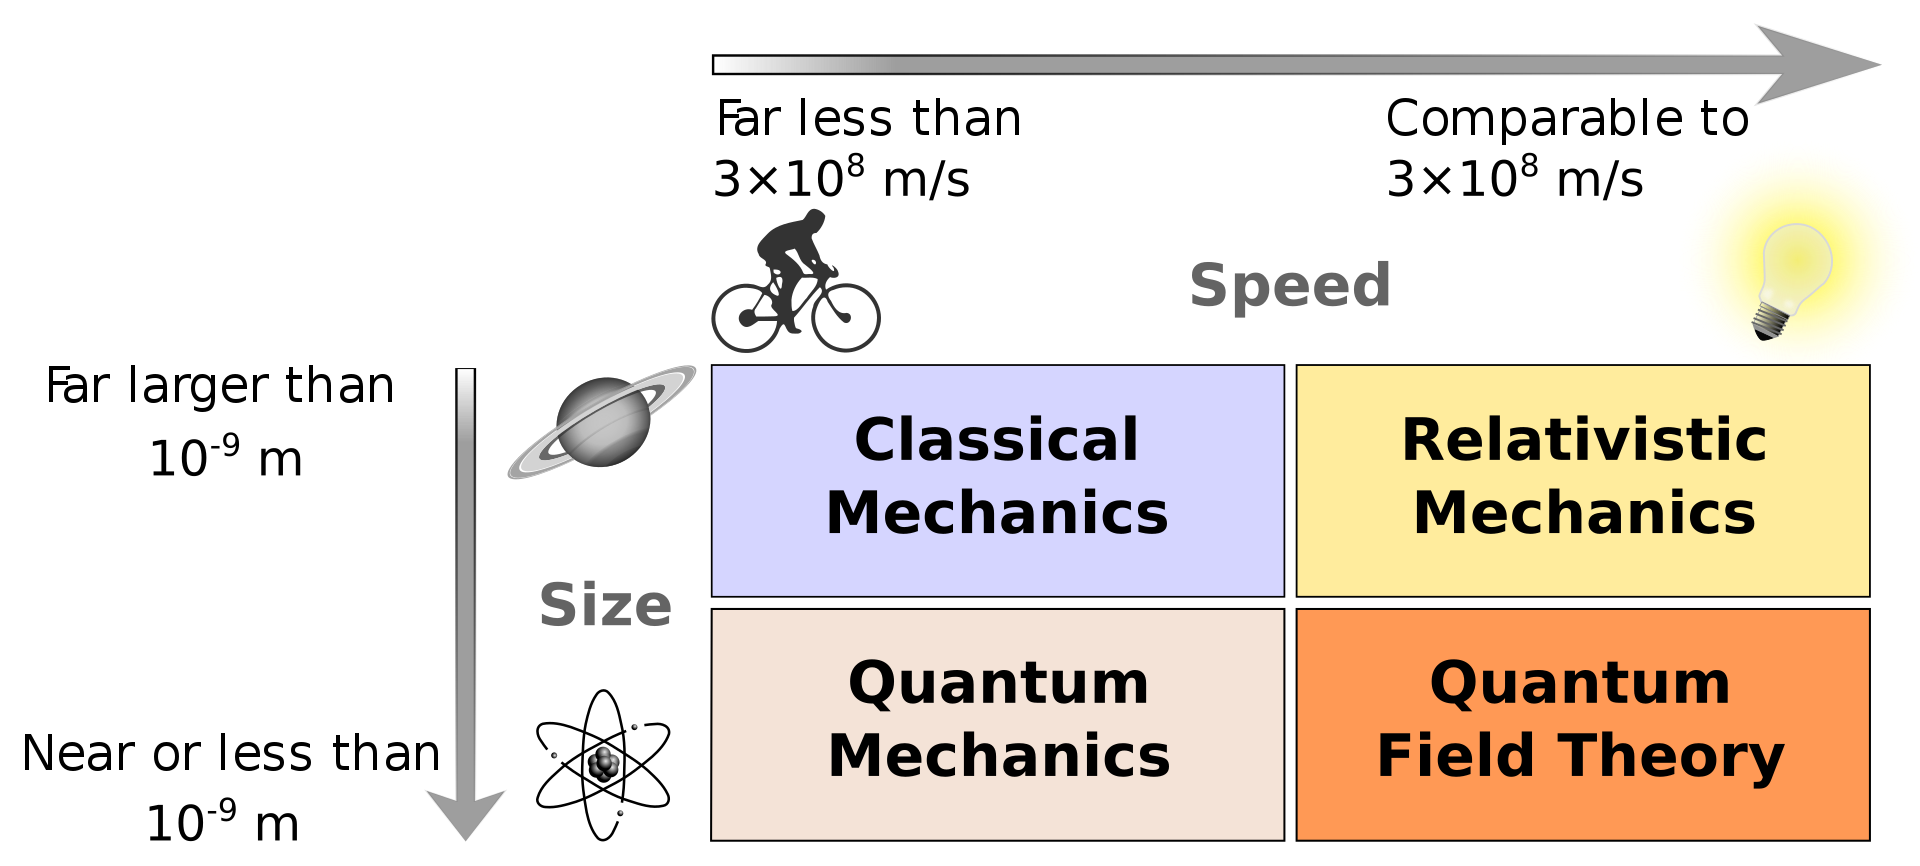
\includegraphics[width=0.5\textwidth]{1920px-Modernphysicsfields.svg.png}
  \caption{Campi della Fisica in relazione a velocità e dimensioni}
\end{wrapfigure}  
Tuttavia, dalle parole di Amaldi del 1955 capiamo che in metà secolo la scienza aveva stravolto il mondo della fisica, mettendo in crisi tutti quelli che costituivano i pilastri della fisica “classica”, come il concetto di tempo assoluto e spazio, la concezione di quiete e moto, il concetto di massa ed energia, il principio di relatività galileana. Nonostante ciò, in realtà, queste scoperte non si rivelarono distruttive nei confronti del passato, ma anzi a completamento delle teorie precedenti. Un completamento che era diventato necessario quando l’indagine dell’uomo si spostò su fenomeni a velocità prossime a quella della luce e soprattutto sul mondo del micro e del macrocosmo. \\

Un esempio pratico ma efficace, per comprendere l’inadeguatezza in certi ambiti del modello classico è quello di un corpo in movimento alla velocità della luce che riflette la sua immagine su di uno specchio. Secondo il modello classico, non esistono velocità assolute ma i corpi si muovono con una velocità relativa rispetto ad un sistema di riferimento, ragione per il quale fu necessaria l’introduzione di un riferimento assoluto e soprattutto immobile rispetto al quale calcolare la velocità di ogni corpo appartenente all’ universo. La quale, fu trovata  nell’\textit{etere}, il quinto elemento, \textit{la quinta essentia}, dopo \textit{il fuoco, l’acqua, la terra e l’aria}, che permea l’intero universo ed è immobile\cite{aristotele}, per l’appunto.  Quindi nel nostro caso, sia il corpo, sia la luce che emette e sia lo specchio, in quanto vincolato al corpo stesso, si muovono ad una velocità c rispetto all’etere. Applicando le trasformazioni galileane rispetto al corpo la velocita della sua luce è $v’= c – U$, ma essendo $U = c$, risulta che la velocità è nulla e che quindi non potrà mai riflettersi sullo specchio.
Inoltre, la considerazione più sconcertante è che nell’ipotesi in cui il corpo fosse un corpo senziente  gli basterebbe guardare nello specchio per rendersi conto di essere in movimento o fermo, nonostante il fatto che si muova secondo un moto rettilineo uniforme. In piena contraddizione con quanto affermava Galileo: \textit{“fate muovere la nave con quanta si voglia velocità; ché
(pur di moto uniforme e non fluttuante in qua e in là) voi non
riconoscerete una minima mutazione in tutti li nominati effetti; né da
alcuno di quelli potrete comprendere se la nave cammina, o pure sta
ferma”}\cite{massimisistemi}.

\section{Relatività ristretta}
\paragraph{I postulati della relatività ristretta}
A differenza delle epoche passate, con la formulazione delle leggi di Maxwell che assegnava alla luce un valore della velocità costante pari a c, diventò di fondamentale importanza la ricerca dell’etere, che fino ad allora era soltanto un’antica teoria mai dimostrata, come sostanza immobile nello spazio assoluto, al fine di non contraddire le leggi della meccanica classica.
Tuttavia, tutti gli esperimenti, compreso il noto esperimento ad opera di Albert Michelson ed Edward Morley, fallirono con la conclusione che l’etere non esistesse. 
Nonostante ciò la scienza doveva trovare una risposta a questo “errore” e vennero pertanto formulate tre possibilità: 
\begin{itemize}
\item Il principio della relativa di Galileo è falso e quindi esiste un modo per rendersi conto se si è fermi o in moto rettilineo uniforme.
\item Le leggi elaborate da Maxwell sono errate e quindi non esiste alcuna costante c.
\item Le trasformazioni di Galileo e la meccanica conseguente sono errate.
\end{itemize}
\medskip
La questione si risolse soltanto nel 1905, con un intuizione geniale da parte di Albert Einstein che trovò consistenza nella formulazione dei due postulati  e della teoria stessa sulla relatività ristretta\cite{einstein}: \\ 

\setlength{\epigraphwidth}{0.8\textwidth}
\epigraph{\textit{“Le leggi secondo cui variano gli stati di un sistema fisico non dipendono dal fatto di essere riferite all’uno o all’altro di due sistemi di coordinate in moto relativo uniforme.”}}{\textbf{Primo postulato}}

\setlength{\epigraphwidth}{0.8\textwidth}
\epigraph{\textit{“Un raggio di luce si muove in ogni sistema inerziale di coordinate con la stessa velocità c, sia che venga emesso da una sorgente fissa o da una sorgente in movimento.”}}{\textbf{Secondo Postulato}}

Il primo postulato non fa altro che confermare il principio di relatività di Galileo è che quindi le leggi fisiche non dipendono dal fatto che siano riferite ad uno o all’altro sistema di coordinate.\\

Il secondo postulato invece afferma chiaramente che la velocità della luce è una costante, il cui valore ($3 \cdot 10^5\: Km/s$) resta immutato in ogni sistema di riferimento che sia esso in moto o fermo. \\

I due postulati, insieme, pesano come macigni sugli equilibri raggiunti dalla fisica fino a quel momento, perché affermare ciò significava mettere in dubbio l’assolutezza che veniva attribuito allo spazio e al tempo. Con questi postulati l’unica cosa assoluta che rimane è soltanto la velocità della luce, in pieno accordo con quanto asserito da Maxwell.
Difatti delle tre possibilità prima elencate, l’unica a rivelarsi vera (o meglio, falsa) è soltanto la terza e infatti si aprì di lì a poco la necessità di nuove trasformazioni che includessero quelle galileane ma che non si limitassero solo ai corpi a velocità molto più bassa di c.

\paragraph{Le trasformazioni di Lorentz}
A differenza delle trasformazioni galileane, le trasformazioni di Lorentz tengono conto non solo delle coordinate spaziali, di un sistema rispetto all’altro ma anche delle coordinate temporali.
Praticamente, se per Galileo il tempo era lo stesso tra un sistema relativo e l’altro quindi $t=t’$, per Lorentz è variabile così come le coordinate spaziali.
Le trasformazioni di Lorentz vengono alla luce nel 1895 con lo scopo di rendere le equazioni di Maxwell valide in tutti i sistemi di riferimento. Tuttavia, è solo grazie alla teoria della relatività ristretta, che esse trovano una giustificazione fisica.\\
Supponendo di avere due sistemi $S$ ed $S’$ formati da tre assi e sia $v$ la velocità di con cui $S'$ si allontana da $S$ sull'asse $x$. Ipotizzando un istante in cui i centri di origine $O$ e $O'$ coincidono e ponendo in questo istante come origine delle coordinate temporali $t=t'=0$, secondo Lorentz:\\
\medskip 

Dati i coefficienti adimensionali:
\begin{center}
\begin{equation}
      \begin{cases}
        \beta = \dfrac{v}{c}\\
        \gamma = \dfrac{1}{\sqrt{1- \beta^2}}
      \end{cases}\,
\end{equation}
\end{center}
\begin{center}
\begin{equation}
\implies
	  \begin{cases}
        x'= \gamma\:(x - v\:t)\\
        y'=y\\
        z'=z\\
        t'=\gamma\:(t-\beta\:\dfrac{x}{c})
      \end{cases}\,
      \qquad \qquad
      \begin{cases}
        x=\gamma\:(x' + v\:t')\\
        y=y'\\
        z=z'\\
        t=\gamma\:(t' + \beta\:\dfrac{x'}{c})
      \end{cases}
\end{equation}
\end{center}

\paragraph{Lorentz e Galileo}-\\
\medskip

Quando $\beta \ll 1$ e quindi $v \ll c$, si può porre: \\
\begin{center}
$\gamma \approx 1 \quad \cup \quad \beta \approx 0 $
\end{center}
Date queste ipotesi, le trasformazioni di Lorentz diventerebbero:
\begin{equation}
	  \begin{cases}
        x'= x - v\:t\\
        y'=y\\
        z'=z\\
        t'=t
      \end{cases}\,
      \qquad \qquad
      \begin{cases}
        x=x' + v\:t'\\
        y=y'\\
        z=z'\\
        t=t'
      \end{cases}
\end{equation}
\textbf{Coincidendo con le trasformazioni di Galileo.}

\section{Dilatazione dei tempi}
\paragraph{I dubbi sulla simultaneità}
Fino ad allora, l’unico modo per stabilire se due eventi stesseri avvenendo simultaneamente o meno era guardarli. Tant’è che per un soggetto senziente basta essere nello stesso luogo in cui i due eventi avvengono per stabilirne un rapporto: che sia esso di simultaneità o di causalità\cite{hume}.
Questa visione, empirica, tuttavia si basa sull’assunto che la velocità della luce sia infinita è che non ci sia ritardo tra il momento in cui essa viene emessa e il momento in cui essa colpisce il nostro occhio. Assunto, che in realtà può essere approssimato a vero, finché le distanze che separano gli eventi sono molto piccole.
Quando invece le distanze toccano gli anni luce è impossibile stabilirne la simultaneità, perché è impossibile stabilire, solo guardando, se la luce che ci è arrivata è vecchia di milioni di anni o di pochi minuti, perché non sappiamo di quanti anni luci era distante la sua sorgente. E quindi due eventi che a noi arrivano simultaneamente probabilmente sono avvenuti in due istanti separati da un intervallo di tempo ad elevato range di variabilità.
Secondo Einstein, l’unico modo per confrontare due eventi distanti nello spazio, sarebbe utilizzare due orologi sincronizzati, con lo stesso meccanismo, posizionati sui due eventi.
Tuttavia, ciò crea un problema. Come si sincronizzano i due orologi se distanti nello spazio? \\
Una soluzione sarebbe utilizzare un mezzo di comunicazione, così che chi imposta l’ora sa in che posizione si trovano le lancette dell’altro orologio. Però, questo sistema trasporta con se un errore, in termini di tempo, che equivale al tempo che l’informazione ha impiegato, muovendosi a cavallo dell’onda radio, per arrivare da un posto all’altro (lag). Allora l’unica soluzione, in questo caso, sarebbe porsi a metà strada tra i due luoghi e comunicare da li, con chi sposta le lancette di entrambi gli orologi finché, \textbf{chi sta in mezzo}, non vede gli orologi segnare la stessa ora.

\begin{wrapfigure}{r}{0.4\textwidth}
  \centering
    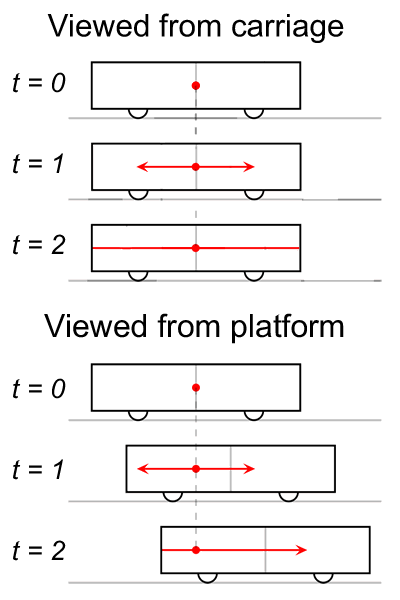
\includegraphics[width=0.35\textwidth]{lAnHM.png}
  \caption{Gedankenexperiment del treno}
\end{wrapfigure}  

\paragraph{Simultaneità relativistica}
Riprendendo  un famoso "gedankenexperiment" (esperimento mentale) elaborato da Einstein, si immagini un treno in movimento a velocità $v$, in cui un osservatore posto al centro di un suo vagone fa partire due raggi di luce, attraverso un laser, rivolti verso le due estremità del vagone esterno.
E si immaginino due sistemi di riferimento $O$ ed $O’$ e due orologi, relativi rispettivamente ad un osservatore esterno in grado di guardare l’interno del vagono, e all’osservatore interno che fa partire i laser.
In questo caso, l’unica cosa vera è che il raggio di luce si muove in ogni caso alla velocità della luce. Tuttavia, mentre per l’osservatore in $O’$, essendo i percorsi che compiono uguali e di conseguenza il tempo che impiegano lo stesso, i due eventi avvengono simultaneamente, per l’osservatore in $O$ le cose non vanno allo stesso modo. Infatti, lui vede una delle code del vagone andare in contro al raggio e un’altra invece scappare dal raggio stesso.  Quindi nello stesso tempo se in un sistema di riferimento i due eventi sono simultanei, in un altro non lo sono più. Questo che per la meccanica classica rappresenterebbe un paradosso è in realtà dovuto al fatto che nonostante per l’osservatore in $O$ la luce si muova in un sistema di riferimento a velocità $v$, la sua velocità risultante non è pari a $u=c+v$ ma in accordo con quanto detto da Einstein, è pari solamente a $u=c$, essendo $c$ una costante invalicabile.

\paragraph{Il paradosso dei gemelli}
Carlo e Franco sono due fratelli gemelli di 25 anni. Nel giorno del loro 25\textsuperscript{o} compleanno Carlo parte per un viaggio spaziale a velocità prossime a quelle della luce $(v=0.98\:c)$. Date queste ipotesi, usciamo dalle leggi della meccanica classica e siamo costretti ad approdare su di un’ottica relativistica diversa. Tant’è che trascurando, il viaggio e le coordinate spaziali in cui si troverà Carlo rispetto a Franco che è rimasto solidale al sistema di riferimento terrestre, si nota che di per certo, date le trasformazioni di Lorentz ogni istante trascorso da Carlo nella navicella sarà diverso da quello trascorso da Franco. Questa affermazione non è altro che una prova del fatto che così come per le coordinate spaziali anche per le coordinate temporali si sono aperte due prospettive  diverse, e infatti dati due istanti:

\begin{center}
$t_1= \dfrac{t'_1 + \dfrac{v\:x'}{c^2}}{\sqrt{1-\dfrac{v^2}{c^2}}} $ \qquad \qquad
$t_2= \dfrac{t'_2 + \dfrac{v\:x'}{c^2}}{\sqrt{1-\dfrac{v^2}{c^2}}} $
\end{center}
Di conseguenza un qualsiasi intervallo di tempo $\Delta t'$ trascorso sulla navicella corrisponde sulla Terra a:
\begin{center}
$\Delta t = t_2 - t_1 = \dfrac{t'_2 + \cancel{\dfrac{v\:x'}{c^2}} - t'_1 - \cancel{\dfrac{v\:x'}{c^2}}}{\sqrt{1-\dfrac{v^2}{c^2}}} = \dfrac{\Delta t'}{\sqrt{1-\dfrac{v^2}{c^2}}}$
\end{center}

Di conseguenza, quando Carlo torna sulla, Terra dopo 10 anni, scopre una sconcertante verità: \textbf{sulla Terra}, sono passati molti più anni. E infatti in accordo con le trasformazioni di Lorentz: 
\begin{center}
$\Delta t = \dfrac{\Delta t'}{\sqrt{1-\dfrac{v^2}{c^2}}} = \dfrac{10\:a}{\sqrt{1 - \dfrac{(0.98\:c)^2}{c^2}}} = 50\:a$
\end{center}
Quindi nel momento del ricongiungimento, quando Carlo ha solo 35 anni, Franco ne ha 75.\\
Un'altra importante considerazione su questo paradosso, riguarda il fatto che entrambi i fratelli, consci della teoria della relatività ristretta, dovrebbero aspettarsi nel momento del ricongiungimento di trovare l'altro fratello più anziano. Ciò in realtà avviene solo per il fratello che ha viaggiato, in quanto il fatto stesso che abbia iniziato "un viaggio" presuppone che da un momento in cui era fermo sulla Terra, abbia accelerato, per poi fermarsi e cambiare rotta, riaccelerando. Sistemi in movimento sottoposti ad accelerazioni non possono essere trattati applicando la relatività ristretta, ma la relatività generale, in cui non si tiene conto solo della meccanica e dell’elettromagnetismo, ma anche della gravità.

\section{Contrazione delle lunghezze}
Così come l'intervallo di tempo tra due istanti, anche la distanza tra due punti è una grandezza relativa.
Infatti, se ipotizziamo 






\chapter{Tempo e anima in S. Agostino}

\chapter{Concezione moderna del tempo}

\chapter{Le metamorfosi di Philip Glass}

 \begin{thebibliography}{12}
\bibitem{Oresme}
  Nicola d'Oresme,
  \textit{Tractatus de configuratione qualitatum et motuum},
  Parigi, XIV secolo.
\bibitem{Metodo}
  René Descartes, \textit{Discorso sul metodo}, Leida, Paesi Bassi, 1637. 
\bibitem{metameditazioni}
  Renè Descartes, \textit{Meditazioni metafisiche}, 1641.
\bibitem{passioni}
  Renè Descartes, \textit{Le passioni dell'anima}, Amsterdam, Paesi Bassi, 1649. 
\bibitem{ragionpura} 
  Immanuel Kant, \textit{Critica della ragion pura}, 1781.
\bibitem{dottrina}  
  Johann Gottlieb Fichte, \textit{La dottrina della scienza}, Jena, Germania, 1794 - 1799.
\bibitem{aristotele}
  Aristotele, \textit{Fisica}, IV secolo a.C. . 
\bibitem{massimisistemi}
  Galileo Galilei, \textit{Dialogo sopra i due massimi sistemi, Giornata seconda}, 1632. 
\bibitem{einstein}
  Albert Einstein, \textit{Elettrodinamica dei corpi in movimento}, Annalen der Physik, Germania, 1905.   
\bibitem{hume}
  David Hume, \textit{Trattato sulla natura umana}, 1739.  
\end{thebibliography}

\end{document}
